\documentclass{article}
\usepackage{graphicx}
\usepackage{hyperref}
\usepackage{amsmath}
\usepackage{times}

\textwidth=6.2in
\textheight=8.5in
%\parskip=.3cm
\oddsidemargin=.1in
\evensidemargin=.1in
\headheight=-0.3in

%------------------------------------------------------------
% newcommand
%------------------------------------------------------------
\newcommand{\scscst}{\scriptscriptstyle}
\newcommand{\scst}{\scriptstyle}
\newcommand{\Robject}[1]{{\texttt{#1}}}
\newcommand{\Rfunction}[1]{{\texttt{#1}}}
\newcommand{\Rclass}[1]{\textit{#1}}
\newcommand{\Rpackage}[1]{\textit{#1}}
\newcommand{\Rexpression}[1]{\texttt{#1}}
\newcommand{\Rmethod}[1]{{\texttt{#1}}}
\newcommand{\Rfunarg}[1]{{\texttt{#1}}}

\usepackage{Sweave}
\begin{document}
\Sconcordance{concordance:warfarinQC.tex:warfarinQC.Rnw:%
1 26 1 1 0 80 1 1 32 4 1 21 0 1 9 3 1 1 11 5 1 1 6 2 1 1 14 27 1 1 18 3 %
1 28 0 1 13 3 1 1 13 30 1 1 0 1 22 3 1 16 0 1 4 1 20 37 1 1 31 1 22 38 %
1 1 40 1 11 54 1 1 28 2 1 1 27 4 1 26 0 1 6 1 22 75 1 1 124 4 1 22 0 1 %
19 7 1 12 0 1 21 41 1 1 0 1 12 9 1 21 0 1 12 2 1 1 10 12 1 1 13 3 1 28 %
0 1 14 5 1 16 0 1 19 14 1 1 16 7 1 1 2 4 1 1 2 4 1 1 2 3 1 1 2 5 1 1 2 %
4 1 1 2 4 1 1 2 29 1}


%------------------------------------------------------------
\title{Aurora Anticoagulation and Anticlotting's EMRs: 
Extraction, Transformation and Loading}
%------------------------------------------------------------
\author{Kourosh Ravvaz}
%\date{}




\maketitle
\tableofcontents

%-------------------------------------------
\section{Introduction}
%--------------------------------------------
The goal of this effort is to extract warfarin treated patients from the Aurora Health Care (AHC) patient database which will be used to create a statistical characterization and use a portion of the patient data to train a Bayesian Network Model to produce accurate Aurora patient population clinical avatar populations. The clinical avatars are used to produce pharmacogenomic simulations to test the predicted accuracy and efficacy outcomes against Aurora Health Care outcome data.

%-------------------------------------------
\section{The Process of Extraction, Transformation, Loading}
%--------------------------------------------
The Aurora Health Care (AHC) project team mined all project data from the Aurora Health Care hospitals and clinics data warehouse for the period of 2002 to 2011. The patient data was de-identified by the AHC project team before distribution to the UWM team.  The UWM team extracted, transformed, and then loaded the de-identified subject records into a working database. The cohort includes patients with evidence of prescription of any of the following medications: Coumadin (Warfarin), Heparin, Ticlopidine (Ticlid), Clopidogrel (Plavix), Dipyridamole (Persantine), Abciximab (ReoPro), Eptifibatide (Integrilin), Tirofiban (Aggrastat), or Dabigatran (Pradaxa).  This effort resulted in a total of 157,450 de-identified data records.  Each data record includes (as available): gender, race, height, weight, age, day of visit, patient\'s zipcode, patient\'s city, provider\'s zipcode, smoking status, INR result, medications received (day, dose, frequency), interacting medications (Amiodarone, Simvastatin, Fluvastatin, Lovastatin, Atrovastatin, Rosuvastatin, Pravastatin, Aspirin), medication indications (by ICD-9 codes: Orthopedic surgery (hip or knee), Deep vein thrombosis, Pulmonary embolism, Atrial fibrillation, Atrial flutter, Atrial fibrillation and flutter, Stroke, Heart valve replacement) and medication adverse events (by ICD-9 codes: Deep vein thrombosis, Pulmonary embolism, Stroke, Myocardial infarction, Bleeding).

The original Aurora Anticoagulation Anticlotting Raw dataset (ARD) was delivered in the MS Access format consisting of the following 12 tables:
\begin{enumerate}
  \item PATIENT AGE
  \item PATIENT GENDER
  \item PATIENT HEIGHTS
  \item PATIENT RACES
  \item PATIENT RESIDENCES
  \item MEDICAL INDICATIONS
  \item INTERACTING MEDICATIONS
  \item ADVERSE EVENTS
  \item MEDICATIONS
  \item INR
  \item PATIENT PROVIDER INFO
  \item PATIENT WEIGHTS
  \item PATIENT TOBACCO USAGE
\end{enumerate}

After a rigorous iterative process of cleaning, transformation and data quality control and assurance, the data was loaded into a working database now called \textbf{WiAD} standing for ``Wisconsin Anticoagulation Anticlotting Database''.  An interactive data profiling and population ``segmentation'' tool \textbf{WiAD-Miner} was developed in R using RStudio and used to facilitate the process of identifying those segments of the total population that satisfied inclusion criteria such as medication name, start-end date of treatment, geographical location (city and county), and number of visits. WiAD-Miner provides a user friendly interactive interface to subset the entire WiAD population and data records and presents a clear view of each extracted subset by producing statistical characteristics and visual profiling (e.g. trend of dose changes during the desired period). The extracted subsets are available for download to conduct further analyses using other tools such as SAS. 

Through the following sections, the process of data cleaning, transformation, and quality control are explained.

%-------------------------------------------
\subsection{Data Transformation and Quality Control}
%--------------------------------------------
The process of data cleaning, data quality control and quality assurance in the context of Aurora electronic medical records (EMR) data reuse for research involves several iterative phases of data analysis and transformation.  Two related approaches for data analysis were taken; a.) data profiling and b.) data mining.  These approaches provide a statistically sound assessment of different aspects of quality at attribute and cross-attribute levels such as completeness, correctness and concordance.

a.) Our data profiling analysis is conducted in three steps.  
\textbf{First}, the method focuses on individual attributes (fields) in the provided dataset.  This step provides a statistically sound assessment of aspects of quality of each attribute including identification of various characteristics of the data such as ``type'', value range, discrete values and their frequency, distribution and variance, uniqueness, occurrence of null values, and the pattern of free text values (e.g., values under ``medication name''). 
\textbf{Second},   the results derived in the first step   are used to handle issues on completeness (e.g., missing values at random, missing values not at random, and partial and complete duplications) by methods such as taking a ``complete case strategy'' limiting the analysis to patients with complete information for all variables, a simple deletion of all incomplete observations and or imputation and to handle issues on correctness (e.g., misspellings, awkward or inaccurate abbreviations, contradictory values, values outside of range, and unexpected changes of sequential data over time) by methods such as transforming and normalizing data elements and prepare them for integration using a data dictionary and looking for elements with values that are outside biologically valid or plausible ranges or that changed questionably or implausibly over time or zero valued elements. 
\textbf{Third}, concordance assessments are done by; a.) Agreement analyses between elements within attributes and b.) Distribution analyses of attributes within the EMR with that of the same information from reference distributions such as similar medical practices, studies or national or state rates (e.g. AHC patient geographical distribution against statewide distributions of race and gender) using both statistical tests and GIS visualizing tools (such as Google Map). Table 1 depicts examples of data problems captured by our data profiling process.

\begin{figure}[ht]
\begin{center}
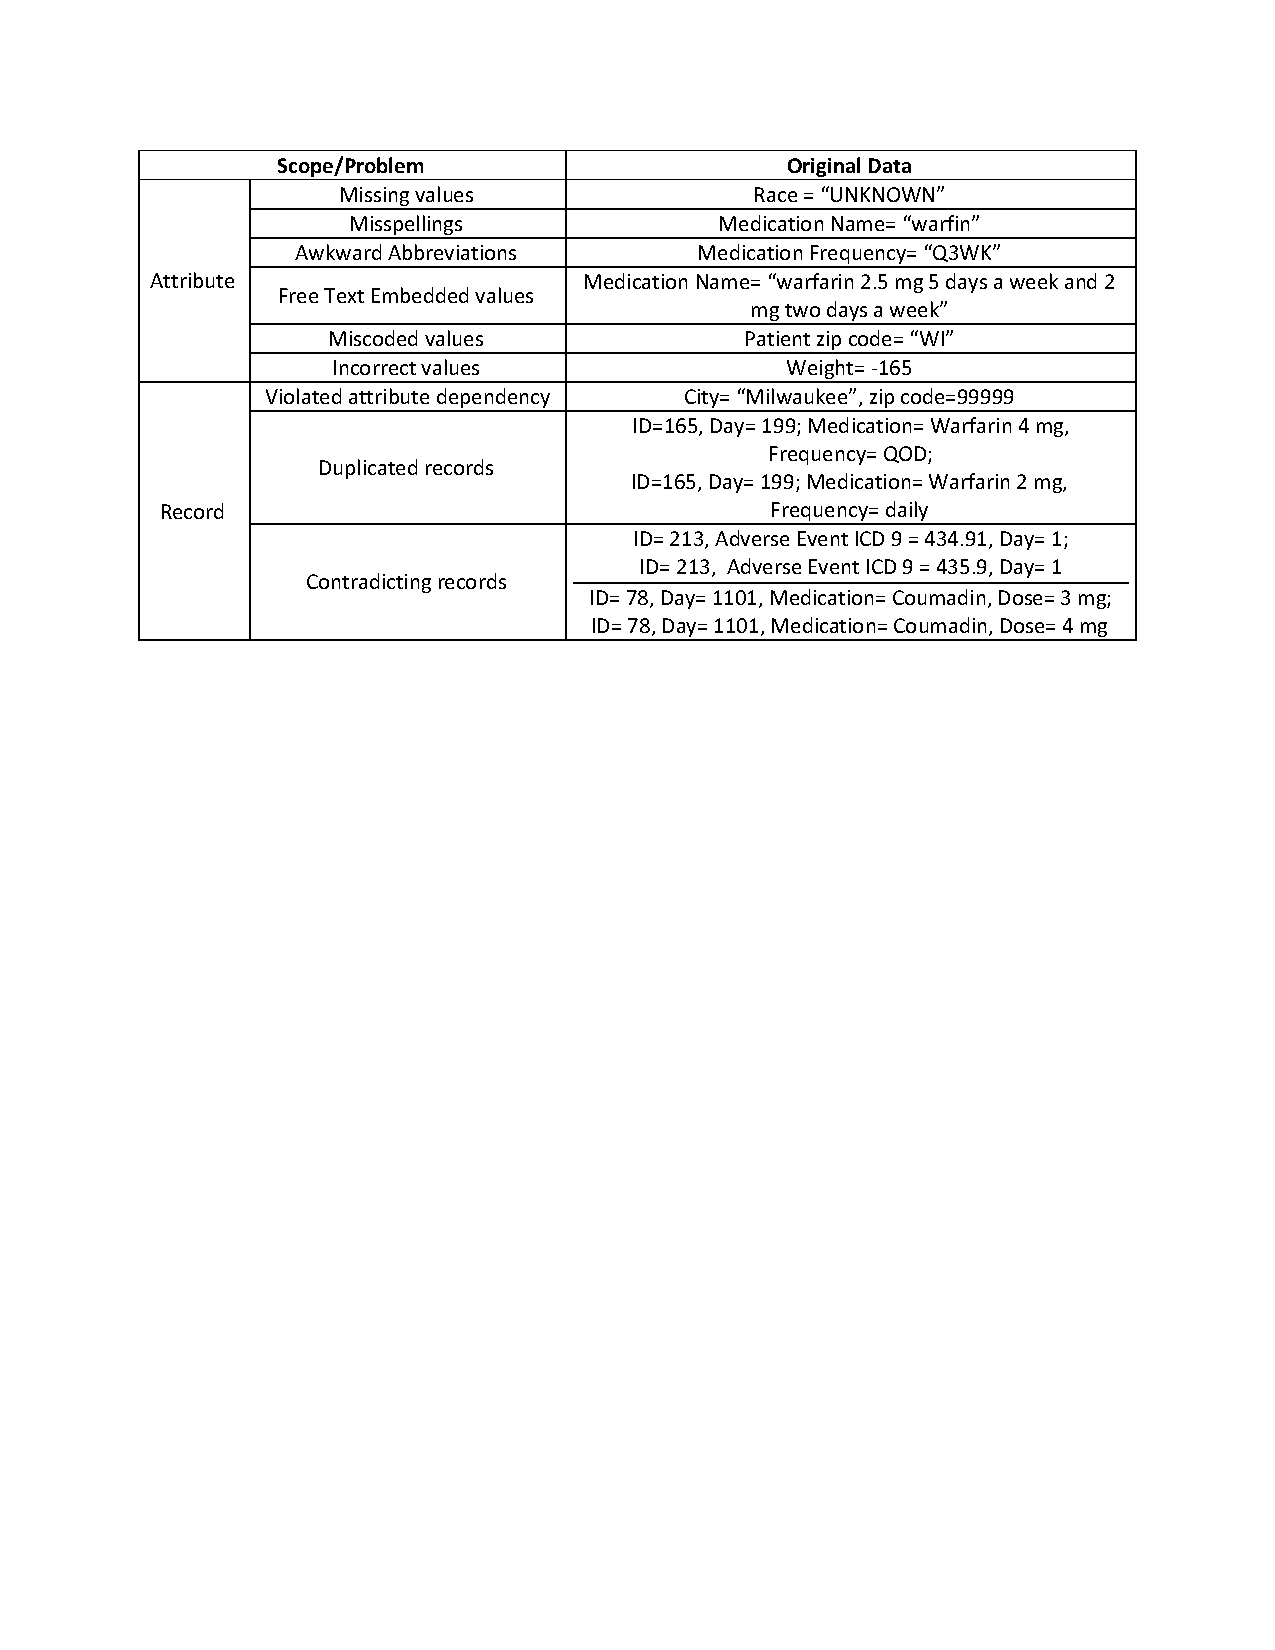
\includegraphics[trim=20mm 165mm 10mm 20mm, clip]{dataQCproblems.pdf}
\caption{Examples for data cleaning and quality control problems.}
\end{center}
\end{figure}

b.) Our robust data mining process also identifies specific data patterns in the data set. Given that this is a temporal and longitudinal dataset, it is very important and useful to take advantage of descriptive data mining models to explore the data more deeply. The models such as clustering, summarization, association discovery and sequence discovery are of interest and applied in this case to explore and evaluate, for example, the pattern of treatment, level of anticoagulation control, and outcome of treatment (e.g., stroke, thromboembolic events, bleeding events, hospitalization, patterns of INR monitoring, and time in the therapeutic range) with different anticoagulation anticlotting agents in patients with different indications.
%-------------------------------------------
\section{General Cleaning and Quality Control}
%--------------------------------------------
In this section, the first round of data cleaning is conducted by taking the following steps on the demographic data: 
\begin{itemize}
  \item First, to identify and exclude records whose attributes' values are missing,
  \item Second, to identify and exclude complete duplicated records,
  \item Third, since in the final modeling and simulation study each subject should have one single value for each demographic characteristics (e.g., weight, height) and given that each subject should have been almost stable in most of the demographic characteristics during the treatment period at AHC, we have to select an aggregation function for obtaining a representative measure of longitudinal records of demographics,
  \item Fourth, to refine the demographic data by excluding highly likely outliers.
\end{itemize}

%-------------------------------------------
\subsection{Age}
%--------------------------------------------
One important point to note is that, although the ARD is a longitudinal  dataset, there is \textbf{only one Gender and one Age record} for each unique subject.

1 subject(s) has missing age information. 2662 subjects have age of 0. Subjects with age of zero or missing age are excluded from the entire study. black list has 2663 and useable list has 154787

Here is the age distribution of the whole ARD population after excluding records with missing age and age of 0.

% latex table generated in R 2.15.2 by xtable 1.7-1 package
% Sun Jul 28 06:26:52 2013
\begin{table}[ht]
\centering
\begin{tabular}{lr}
  \hline
Age.Range & Percentage \\ 
  \hline
$<$18 & 0.23 \\ 
  18-24 & 0.86 \\ 
  25-34 & 2.46 \\ 
  35-44 & 5.81 \\ 
  45-54 & 14.11 \\ 
  55-59 & 9.92 \\ 
  60-64 & 10.62 \\ 
  65-74 & 22.22 \\ 
  75-84 & 22.70 \\ 
  $>$85 & 11.08 \\ 
   \hline
\end{tabular}
\caption{Age Distriubtion of the Aurora Raw Data} 
\label{Table:3}
\end{table}

\begin{figure}
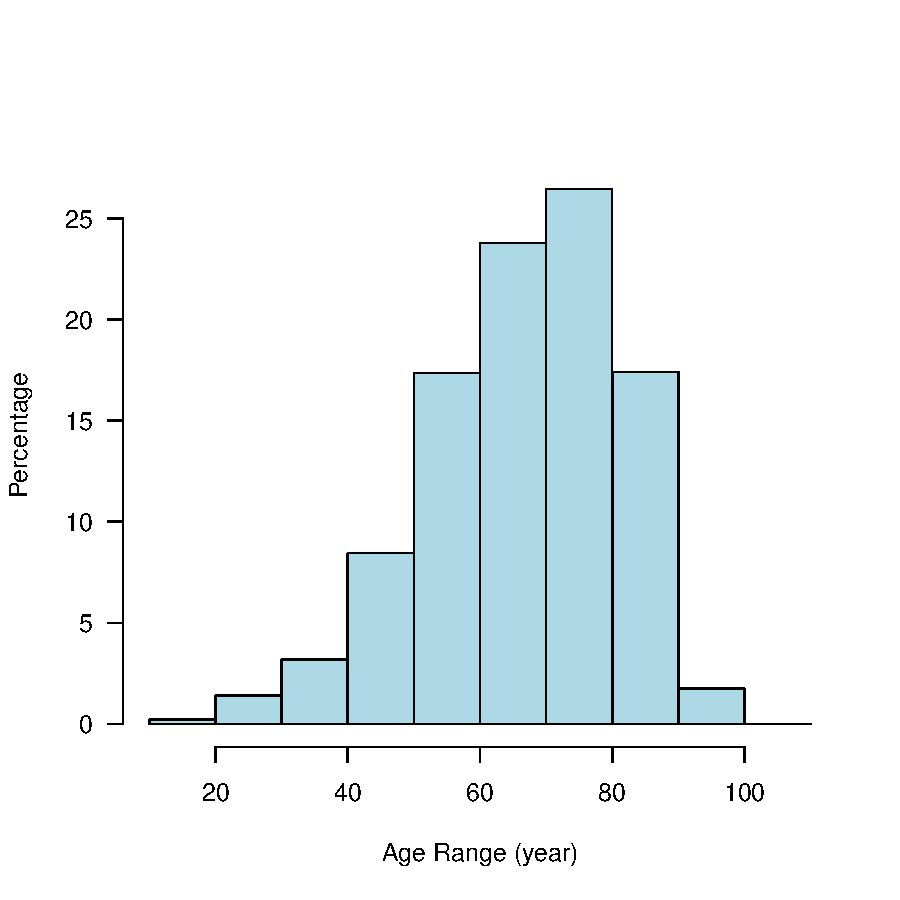
\includegraphics{Fig-fig1}

\caption{ARD Population - Age Distribution}

\end{figure}
\newpage

The number of subjects in whole poulation with an age under 18 is 357 .The number of subjects in whole poulation with an age over 100 is 65 .The number of subjects in whole poulation with an age over 110 is 1 .
\textbf{The subjects with age of 18 or lower are excluded from the study population as our study's age inclusion criteria is age 18 and over.}

black list has 3020 and useable list has 154430 .

\begin{quote}
\textbf{Quality Assessment Summary:}
\end{quote}
\begin{quote}
\emph{Strength:}
\end{quote}
\begin{itemize}
  \item Duplication: Each subject has just one age record (no duplicated age records).
  \item Complemetness: 1.69\% of the whole population (2663 subjects) have missing age information.
  \item Accuracy: Number of subjects with age over 100 and 110 are 0.04\% (65 subject) and less than 0.001\% (1 subject). Given the oldest person lived in Wisconsin was 112 years old, the percentage of outlier ages is very low.
  \item The Age distrubution of the subjects is skewed to right as expected.
\end{itemize}
\begin{quote}
\emph{Weakness:}
\end{quote}
\begin{itemize}
  \item Consistency: Since there is just one age record for each subject, it is not possible to check any inconsistency whithin age records of each subject.
  \item Accuracy: Even though not requested, 357 subjects with an age under 18 were included in the provided dataset.
\end{itemize}

\textbf{After cleaning and qulaity control of the age attribute, the number of the remaining subjetcs is 154,430 (98.08\% of the total).} 

%-------------------------------------------
\subsection{Gender}
%--------------------------------------------

16 subjects have missing gender information.
Here is the gender distribution of the ARD (Table 4) and also that of Milwaukee County and the State of Wisconsin (Table 5) for comparison. 

% latex table generated in R 2.15.2 by xtable 1.7-1 package
% Sun Jul 28 06:26:53 2013
\begin{table}[ht]
\centering
\begin{tabular}{lr}
  \hline
Gender & Percentage \\ 
  \hline
Male & 50.34 \\ 
  Female & 49.65 \\ 
  Missing & 0.01 \\ 
   \hline
\end{tabular}
\caption{Gender Distriubtion in the Aurora Raw Data} 
\label{Table:1}
\end{table}% latex table generated in R 2.15.2 by xtable 1.7-1 package
% Sun Jul 28 06:26:53 2013
\begin{table}[ht]
\centering
\begin{tabular}{rrr}
  \hline
 & MKE(\%) & WI(\%) \\ 
  \hline
Male & 48.30 & 49.60 \\ 
  Female & 51.70 & 50.40 \\ 
   \hline
\end{tabular}
\caption{Gender Distriubtion in Milwaukee County (MKE) and Wisconsin (WI).} 
\label{Table:1}
\end{table}

\textbf{The subjects with missing gender are excluded from the study population.}

black list has 3036 and useable list has 154414 .
\newpage

\begin{quote}
\textbf{Quality Assessment Summary:}
\end{quote}
\begin{quote}
\emph{Strength:}
\end{quote}
\begin{itemize}
  \item Duplication: No duplicated gender records.
  \item Complemetness: Almost whole the pouplation (except 16 subjects) have gender information.
  \item Accuracy: The gender distribution is very much consistent with that of Milwaukee County and State of Wisconsin.
\end{itemize}
\begin{quote}
\emph{Weakness:}
\end{quote}
\begin{itemize}
  \item Consistency: Since there is just one gender record for each subject, it is not possible to check any inconsistency whithin gender records of each subject.
\end{itemize}

\textbf{After cleaning and qulaity control of the gender attribute, the number of the remaining subjetcs is 154,414 (98.07\% of the total).} 

%-------------------------------------------
\subsection{Race}
%--------------------------------------------
In the ARD, each subject has one race record. Race has the following attributes:
SURROGATE\_ID, RACE, SOURCE\_SYSTEM.
Since race is a required information for the future analysis, I have to check to make sure if there is any subject with missing race information and if so exclude them.

Race types are: White, Black or African American, UNKNOWN, Asian,
American Indian or Alaskan Native, Native Hawaiian/Other Pacific
Islander .1662 subjects have UNKNOWN race information. 52.85 percent of the whole population have race information.
The following table depics the race distribution of the ARD population.

% latex table generated in R 2.15.2 by xtable 1.7-1 package
% Sun Jul 28 06:26:54 2013
\begin{table}[ht]
\centering
\begin{tabular}{lr}
  \hline
Race & Percentage \\ 
  \hline
White & 90.41 \\ 
  Black or African American & 8.52 \\ 
  Asian & 0.79 \\ 
  American Indian or Alaskan Native & 0.27 \\ 
  Native Hawaiian/Other Pacific Islander & 0.02 \\ 
   \hline
\end{tabular}
\caption{Race Distriubtion in the Aurora Raw Data} 
\label{Table:3}
\end{table}
black list has 4559 and useable list has 80885 .

\begin{quote}
\textbf{Quality Assessment Summary:}
\end{quote}
\begin{quote}
\emph{Strength:}
\end{quote}
\begin{itemize}
  \item Duplication: No duplicated race records.
  \item Complemetness: 1.9\% of the subjects with race information have race record of "UNKNOWN".
  \item Accuracy: The percentages of White and African-American among the subjects with race information are approximately equal to those for State of Wisconsin.
\end{itemize}
\begin{quote}
\emph{Weakness:}
\end{quote}
\begin{itemize}
  \item Completeness: 52.85\% of the whole population have race information.
  \item Accuracy: Since there is just one race record for each subject, it is not possible to check the accuracy of the race information for each subject.
\end{itemize}

\textbf{After cleaning and qulaity control of the race attribute, the number of the remaining subjetcs is 80,885 (51.37\% of the total).} 


%-------------------------------------------
\subsection{Height}
%--------------------------------------------
In the ARD, each subject has multiple height records. Height has the following attributes:
SURROGATE\_ID, EFFECTIVE\_DAY, HEIGHT, SOURCE\_SYSTEM.

For the height records, a few steps are taken:
\begin{itemize}
  \item First, to identify and exclude height records whose HEIGHT attributes are missing.
  \item Second, to identify and exclude duplicated height records.
  \item Third, since in the final modeling and simulation study each subject should have one height record and given that each subject should have been almost stable in height during the treatment period at AHC, we take the median of each subject's height records and take it as the representative height of the subject. 
  \item Fourth, the height medians are refined by excluding the ones that here are considered outliers (i.e., median heights over or lower than 3 standard deviations). 
\end{itemize} 

Heights records include 333385 duplicate records.The ARD poulation on average has 3.07 height records/subject.The average height of the original poulation is 66.09 inch.  938 have outlier height. 
black list has 4612 subjects and useable list has 63550 subjects.

\begin{quote}
\textbf{Quality Assessment Summary:}
\end{quote}
\begin{quote}
\emph{Strength:}
\end{quote}
\begin{itemize}
  \item Duplication: No duplicated race records.
  \item Complemetness: 1.9\% of the subjects with race information have race record of "UNKNOWN".
  \item Accuracy: The percentages of White and African-American among the subjects with race information are approximately equal to those for State of Wisconsin.
\end{itemize}
\begin{quote}
\emph{Weakness:}
\end{quote}
\begin{itemize}
  \item Completeness: 52.85\% of the whole population have race information.
  \item Accuracy: Since there is just one race record for each subject, it is not possible to check the accuracy of the race information for each subject.
\end{itemize}


\textbf{After cleaning and qulaity control of the height attribute, the number of the remaining subjetcs is 63,550 (40.36\% of the total).}

%-------------------------------------------
\subsection{Weight}
%--------------------------------------------
In the ARD, each subject has multiple weight records. Weight has the following attributes:
SURROGATE\_ID, EFFECTIVE\_DAY, WEIGHT, SOURCE\_SYSTEM.

For the weight records, a few steps are taken:
\begin{itemize}
  \item First, to identify and exclude weight records whose WEIGHT attributes are missing.
  \item Second, to identify and exclude duplicated weight records.
  \item Third, since in the final modeling and simulation study each subject should have one weight record and given that each subject should have been almost stable in weight during the treatment period at AHC, we take the median of each subject's weight records and take it as the representative weight of the subject. 
  \item Fourth, the weight medians are refined by excluding the ones that here are considered outliers (i.e., median weights over or lower than 3 standard deviations). 
\end{itemize}


Weights records include 61312 duplicate records.The ARD poulation on average has 7.39 weight records/subject.The average weight of the original poulation is 195.12 pound.  79 have outlier weight. 
black list has 4668 subjects and useable list has 62504 subjects.

\begin{quote}
\textbf{Quality Assessment Summary:}
\end{quote}
\begin{quote}
\emph{Strength:}
\end{quote}
\begin{itemize}
  \item Duplication: No duplicated race records.
  \item Complemetness: 1.9\% of the subjects with race information have race record of "UNKNOWN".
  \item Accuracy: The percentages of White and African-American among the subjects with race information are approximately equal to those for State of Wisconsin.
\end{itemize}
\begin{quote}
\emph{Weakness:}
\end{quote}
\begin{itemize}
  \item Completeness: 52.85\% of the whole population have race information.
  \item Accuracy: Since there is just one race record for each subject, it is not possible to check the accuracy of the race information for each subject.
\end{itemize}


\textbf{After cleaning and qulaity control of the weight attribute, the number of the remaining subjetcs is 62,504 (39.69\% of the total).}


%-------------------------------------------
\subsection{Tobacco Use}
%--------------------------------------------
In the ARD, each subject has multiple ``Tobacco Use'' records as this information was recorded on different days of visit. The records have the following attributes:
SURROGATE\_ID, EFFECTIVE\_DAY, TOBACCO\_USE, SOURCE\_SYSTEM.

For the Tobacco Use records, a few steps are taken:
\begin{itemize}
  \item First, to identify and exclude Tobacco Use records whose TOBACCO\_USE attributes are missing.
  \item Second, to identify and exclude duplicated records.
  \item Third, to identify and exclude non-sense records.
  \item Fourth, to normalize and transform the values under attribute TOBACCO\_USE using a dictionary.
  \end{itemize}
  
\begin{quote}
\textbf{Non-sense or inaccurate records:}
\end{quote}
In some records, TOBACCO\_USE values are not relevant or accurate such as the followings:
``admit to icu'', ``30 day readmit'', and ``already done''. Any record with such TOBACCO\_USE values are deleted.

\begin{quote}
\textbf{Normalization and Transformation:}
\end{quote}
Relevant TOBACCO\_USE values are not consistent in terms of spelling and format. After normalization, a dictionary is used to translate and transform the values to those of desired for the modeling and simulation study. Each reported sensible TOBACCO\_USE value is translated into one of the followings: current, not-current, never, or unknown. 
Majority of subjetcs have the same tobacco use behavior during the course of their treatment. In some subjects, the tobacco use behavior has changed over time. The reported tobacco use behavior of some subjects looks conflicting. For instance, both records ``Current''  and ``Never'' were reported for some subjects.

\textbf{This white paper explores the butterfly effect of poor data quality on CRM, ERP, billing, data 
warehouse, and other enterprise systems.}







The following table shows the distribution of tobacco use values for the subjects with that information. 

% latex table generated in R 2.15.2 by xtable 1.7-1 package
% Sun Jul 28 06:28:37 2013
\begin{table}[ht]
\centering
\begin{tabular}{cc}
  \hline
 & Number of Subjects \\ 
  \hline
Current & 15040 \\ 
  Not\_current & 33109 \\ 
  Never & 42941 \\ 
  Unknown & 188 \\ 
  Current \& Not\_current & 3125 \\ 
  Current \& Never & 716 \\ 
  Current \& Unknown & 121 \\ 
  Not\_current \& Never & 9713 \\ 
  Not\_current \& Unknown & 243 \\ 
  Never \& Unknown & 403 \\ 
  Current, Not\_current \& Never & 725 \\ 
  Current, Not\_current \& Unknown &  46 \\ 
  Current, Never \& Unknown &  18 \\ 
  Not\_current, Never \& Unknown & 232 \\ 
  Current, Not\_current, Never \& Unknown &  50 \\ 
   \hline
\end{tabular}
\caption{Distribution of Combination of Tobacco Use Values.} 
\label{Table:1}
\end{table}
black list has 5301 subjects and useable list has 61565 subjects.
The subjects with any of the following reported combination of tobacco use bahaviors were excluded: ``Current \& Never'', ``Current, Not current \& Never'', ``Current, Never \& Unknown'', and ``Current, Not current, Never \& Unknown''. 


\begin{quote}
\textbf{Quality Assessment Summary:}
\end{quote}
\begin{quote}
\emph{Strength:}
\end{quote}
\begin{itemize}
  \item Duplication: The percentage of duplicated records is very low.
  \item Accuracy: A small number of subjects with tobacco use information have non-sensible information (0.59\%). 
  \item The reported changes of tobacco use behavior of majority of the subjects look consistent. 
\end{itemize}
\begin{quote}
\emph{Weakness:}
\end{quote}
\begin{itemize}
  \item Completeness: 67.74\% (106,670 subjects) of the whole population have sensible tobacco use information.
  \item Accuracy: The reported change of tobacco use behavior of 1509 subjects over time looks conflicting (1.4\%). 
\end{itemize}


\textbf{After cleaning and qulaity control of the tobacco use attribute, the number of the remaining subjetcs is 61,565 (39.10\% of the total).}





%-------------------------------------------
\section{General Overview of the Medications Records}
%--------------------------------------------
The Auroa Raw Dataset (ARD) includes 2,349,633 longitudinal medication records representing 157,450 unique subjects. As a result of being a longitudinal dataset, each subject has more than one medication record. 

%-------------------------------------------
\subsection{Medications Records' Attributes}
%--------------------------------------------
Each medication record has the following attributes:
\begin{itemize}
  \item SURROGATE\_ID
  \item DAY\_PRESCRIBED
  \item MEDICATION\_NAME
  \item FREQ, 
  \item DOSE\_QTY
  \item DOSE\_QTY\_UNIT
  \item SOURCE\_SYSTEM
\end{itemize}


%-------------------------------------------
\subsection{Distribution of Medications Records}
%--------------------------------------------
First, I have to identify any specific medication cohort by extracting any records in the Aurora Raw Dataset (ARD)'s Medications records including any of the following terms:
\begin{itemize}
  \item Warfarin or Coumadin
  \item Heparin
  \item Clopidogrel or Plavix
  \item Dabigatran or Pradaxa
  \item Eptifibatide or Integrilin
  \item Abciximab or ReoPro
  \item Ticlopidine or Ticlid
  \item Tirofiban or Aggrastat
  \item Dipyridamole or Persantine
\end{itemize}

After identifying the records, they have to be cleaned and transfomred for the following issues:
\begin{itemize}
  \item Duplications
  \item Free Text Embedded values
\end{itemize}

The free text embedded values of the medication cohorts are used to extract dosage, unit, and route.

Then the next step is to take a strategy on how to deal with the incomplete records as we need records including name of the medication, day prescribed, frequency of the medication, dosage of the medication, unit, and probably medication route.

1375397 medications records have missing Frequency information. 
Here is the medications records distribution by medication.


% latex table generated in R 2.15.2 by xtable 1.7-1 package
% Sun Jul 28 06:30:27 2013
\begin{table}[ht]
\centering
\begin{tabular}{lp{2cm}p{2cm}p{2cm}p{2cm}}
  \hline
 & Records with med. name(\%) & Subjects with med. name(\#) & Records with med. name \& dose(\%) & Subjects with dose(\#) \\ 
  \hline
Warfarin & 37.85 & 74102 & 11.00 & 51896 \\ 
  Heparin & 36.24 & 71537 & 2.31 & 23899 \\ 
  Clopidogrel & 24.93 & 61517 & 5.17 & 41851 \\ 
  Dabigatran & 0.30 & 1793 & 0.13 & 1599 \\ 
  Dipyridamole & 0.27 & 2192 & 0.05 & 525 \\ 
  Eptifibatide & 0.19 & 3066 & 0.15 & 2886 \\ 
  Ticlopidine & 0.14 & 434 & 0.04 & 310 \\ 
  Abciximab & 0.08 & 1310 & 0.05 & 1181 \\ 
  Tirofiban & 0.00 & 48 & 0.00 & 0 \\ 
   \hline
Total & 100.00 & 215999 & 18.90 & 124147 \\ 
   \hline
\end{tabular}
\caption{Medications Records Distriubtion by Medication.} 
\label{Table:1}
\end{table}


99.02\% of the medications records includes one of the three medications of Warfarin (37.85\%), heparin (36.24\%) and clopidogrel (24.93\%). Warfarin records which have dosage information have the highest percentage of whole the records (11\%). Although the number of heparin records is bigger than the number of clopidogrel records, the percentage of clopidogrel records with dosage information out of whole the records is higher than that of heparin.
The above table indicates that a big number of subjects have received more than one medication. The following table shows the number of subjects who have been under treatment with 1 to 6 medications.


% latex table generated in R 2.15.2 by xtable 1.7-1 package
% Sun Jul 28 06:30:27 2013
\begin{table}[ht]
\centering
\begin{tabular}{lrrrrrr}
  \hline
Number of Medications & 1 & 2 & 3 & 4 & 5 & 6 \\ 
  \hline
Number of Subjects & 75282 & 16441 & 3049 & 358 &  20 &   1 \\ 
   \hline
\end{tabular}
\caption{Number of Subjects by Number of Received Medications - Only medication records with dosage information included.} 
\label{Table:1}
\end{table}
\newpage

\begin{quote}
\textbf{Quality Assessment Summary:}
\end{quote}
\begin{quote}
\emph{Strength:}
\end{quote}
\begin{itemize}
  \item Duplication: 20\% of the medication records are duplicated records (by attributes SURROGATE\_ID, DAY\_PRESCRIBED, and MEDICATION\_NAME). In some cases, they are useful for accuracy check. 
  \item Complemetness: All the subjects have medications records.
\end{itemize}
\begin{quote}
\emph{Weakness:}
\end{quote}
\begin{itemize}
  \item Completeness: None of the medication records has any structured information on Dose Quantity and Dose Unit. These pieces of information are embedded in free text under attribute "Medication Name".
  \item The information on "SOURCE SYSTEM" is incomplete as all of them are reported "legacy".
  \item 58.53\% of medication records do not have Frequency information (1,375,397 out of 2,349,633 records). 
  \item Duplication: 20\% of the medication records are duplicated records (by attributes SURROGATE\_ID, DAY\_PRESCRIBED, and MEDICATION\_NAME).
  \item Accuracy: The records of the same day are inconsistent in a number of cases. This is studied in detail for each medication.
\end{itemize}


\textbf{After cleaning and qulaity control of the height attribute, the number of the remaining subjetcs is 63,550 (40.36\%).}



%-------------------------------------------
\section{Warfarin Cohort}
%--------------------------------------------
Given that each medication has specific characteritsics, the analysis of each medication is done separately after general anaysis done on all of the records.
Warfarin cohort has the biggest number of records in the ARD and is also the medication of interest for the first modeling and simulation study. So, the analysis of this cohort's records is done first.  

%-------------------------------------------
\subsection{Warfarin Cohort's Demographics}
%--------------------------------------------

The warfarin cohort implies warfarin and coumadin records with at least one piece of dosage information and age, gender, race, height and weight information.

The warfarin cohort includes 186 records which have more than one embedded digit 
(e.g., warfarin 2.5 mg 5 days a week and 2 mg two days a week). 
To take advanatage of these records, they should be manually cleaned and transformed.   

%-------------------------------------------
\subsubsection{Age}
%--------------------------------------------

Here is the age distribution of the warfarin cohort after excluding records with missing age and age of 0.


% latex table generated in R 2.15.2 by xtable 1.7-1 package
% Sun Jul 28 06:30:29 2013
\begin{table}[ht]
\centering
\begin{tabular}{lr}
  \hline
Age.Range & Percentage \\ 
  \hline
$<$18 & 0.00 \\ 
  18-24 & 0.63 \\ 
  25-34 & 1.93 \\ 
  35-44 & 4.71 \\ 
  45-54 & 12.25 \\ 
  55-59 & 9.19 \\ 
  60-64 & 10.69 \\ 
  65-74 & 25.36 \\ 
  75-84 & 25.65 \\ 
  $>$85 & 9.60 \\ 
   \hline
\end{tabular}
\caption{Age Distriubtion in the Aurora Raw Data - Warfarin Cohort} 
\label{Table:4}
\end{table}
\begin{figure}
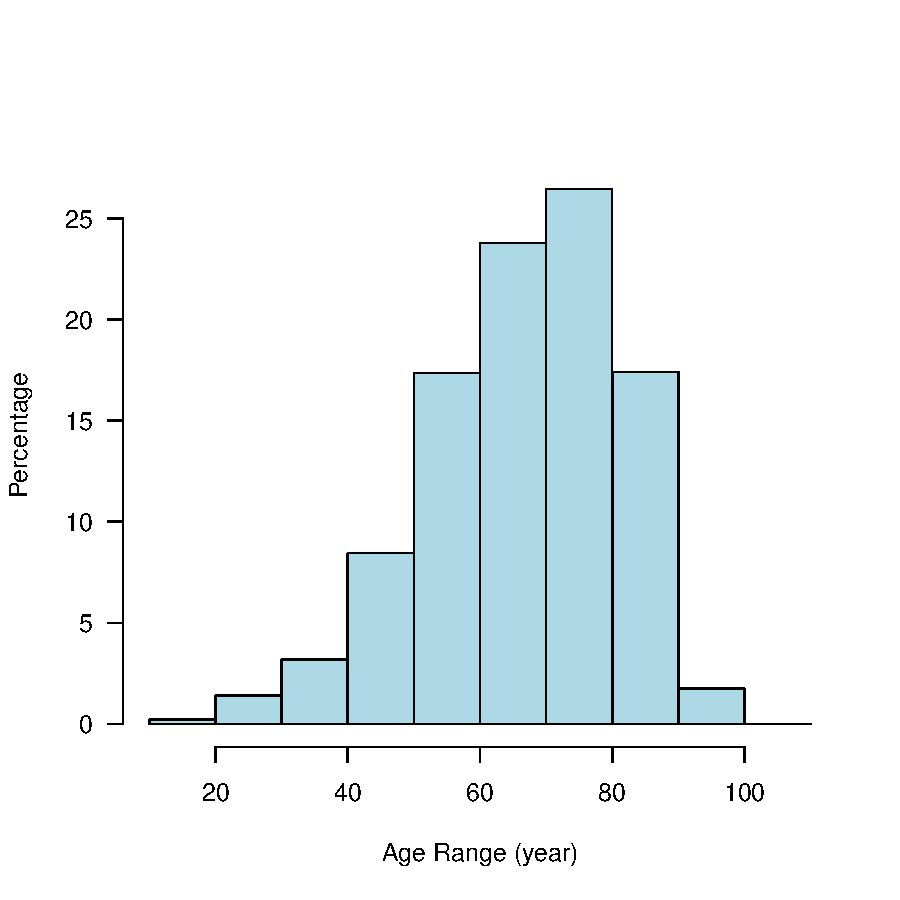
\includegraphics{Fig-fig1}

\caption{Warfarin Cohort - Age Distribution}

\end{figure}
\newpage




%-------------------------------------------
\subsubsection{Gender}
%--------------------------------------------


Here is the gender distribution of the warfarin cohort (Table 4) and also that of Milwaukee County and the State of Wisconsin (Table 5) for comparison. 

% latex table generated in R 2.15.2 by xtable 1.7-1 package
% Sun Jul 28 06:30:30 2013
\begin{table}[ht]
\centering
\begin{tabular}{lr}
  \hline
Gender & Percentage \\ 
  \hline
Male & 51.02 \\ 
  Female & 48.98 \\ 
  Missing & 0.00 \\ 
   \hline
\end{tabular}
\caption{Gender Distriubtion in the Aurora Raw Data - Warfarin Cohort} 
\label{Table:1}
\end{table}% latex table generated in R 2.15.2 by xtable 1.7-1 package
% Sun Jul 28 06:30:30 2013
\begin{table}[ht]
\centering
\begin{tabular}{rrr}
  \hline
 & MKE(\%) & WI(\%) \\ 
  \hline
Male & 48.30 & 49.60 \\ 
  Female & 51.70 & 50.40 \\ 
   \hline
\end{tabular}
\caption{Gender Distriubtion in Milwaukee County (MKE) and Wisconsin (WI).} 
\label{Table:1}
\end{table}%-------------------------------------------
\subsubsection{Race}
%--------------------------------------------
The following table shows the race distribution of the warfarin cohort.

% latex table generated in R 2.15.2 by xtable 1.7-1 package
% Sun Jul 28 06:30:31 2013
\begin{table}[ht]
\centering
\begin{tabular}{lr}
  \hline
Race & Percentage \\ 
  \hline
White & 93.96 \\ 
  Black or African American & 5.39 \\ 
  Asian & 0.47 \\ 
  American Indian or Alaskan Native & 0.16 \\ 
  Native Hawaiian/Other Pacific Islander & 0.02 \\ 
   \hline
\end{tabular}
\caption{Warfarin Cohort's Race Distriubtion} 
\label{Table:3}
\end{table}\newpage

%-------------------------------------------
\subsubsection{Height}
%--------------------------------------------
In the ARD, each subject has multiple height records. Height has the following attributes:
SURROGATE\_ID, EFFECTIVE\_DAY, HEIGHT, SOURCE\_SYSTEM

For the height records, a few steps are taken:
First, to identify and exclude height records whose HEIGHT attributes are missing.
Second, to identify and exclude duplicates height records.
Third, since in the final modeling and simulation study each subject should have one height record and given that each subject should have been almost stable in height during the treatment period at AHC, we take the median of each subject's height records and take it as the height of the subject. Third, the height medians are refined by excluding the ones that here are considered outliers (i.e., median heights over or lower 3 standard deviations). 
Fourth, to identify and extract the height of warfarin cohort.
 

The average height of the warfarin cohort after excluding the outliers is 66.98 inch.



%-------------------------------------------
\subsubsection{Weight}
%--------------------------------------------


%-------------------------------------------
\subsubsection{Residence}
%--------------------------------------------


%-------------------------------------------
\subsubsection{Tobacco Use}
%--------------------------------------------


%-------------------------------------------
\subsection{Warfarin Cohort's Clinical Characteristics}
%--------------------------------------------


%-------------------------------------------
\subsubsection{INR}
%--------------------------------------------


%-------------------------------------------
\subsubsection{Medical Indications}
%--------------------------------------------


%-------------------------------------------
\subsubsection{Adverse Events}
%--------------------------------------------


%-------------------------------------------
\section{Heparin Cohort}
%--------------------------------------------

%-------------------------------------------
\section{Clopidogrel Cohort}
%--------------------------------------------


%-------------------------------------------
\section{Dabigatran Cohort}
%--------------------------------------------

%-------------------------------------------
\section{WiAD-Miner}
%--------------------------------------------


%------------------------------------
\section{Reference}
%-------------------------------------


\end{document}





